\chapter{Software}
%not sure if use-cases should not go into a different chapter\\
%this chapter would then focus on just the process of developing my analysis pipeline and finish with a detailed description of it.

\begin{comment}
TODO:\\
-Add what I did: somewhat detailed description of my process in developing the notebook\\
-start from the notebook which was started by Radomir for custom structure (before openMNGlab)\\
-adding of importers from old openMNGlab version (code from Fabian)\\
-adding of neo importers after integration into openMNGlab\\

-Explain the details of the different structures in python (recording from old version, neo recording/block/segment, csv files)\\
-add diagram of big picture structure of openMNGlab in greater spike data analysis pipeline\\
\end{comment}

\section{Data structure}
In this section I will present the details of the different data structures that I will use in the course of my analysis pipeline.

\subsection{Neo structure}
Neo models electrophysiological data in a hierarchical structure, which is depicted in Figure~\ref{fig:neostructure}. On the lowermost level we start with data objects. An AnalogSignal is regularly sampled data and can contain multiple channels. An IrregularlySampledSignal is similar, but does not feature a regular sampling interval, as the name suggests. A SpikeTrain object contains time point data with th information when action potentials occur. These SpikeTrain objects are, however, slightly different from our understanding of spike trains in this thesis. We understand a spike train as the spikes that occur resulting from one stimulus and is quite limited duration wise. The SpikeTrain object in the Neo structure is a collection of all spikes during one recording and all spike trains as we see them would be contained in one such SpikeTrain object.\\
Events in Neo point to distinct points in time and can be used to mark stimulation events for experiments with animals for example. Epochs function similar to events, but cover a duration instead of just points in time.\\
On the next layer up there are objects for grouping all of these lower level objects. The first of these objects is a Segment. This groups data that was simultaneously recorded. Then there are so called Groups which can group data in any arbitrary way and is not restricted to the data being  in the same Segment. On the topmost layer there are Blocks. One block contains multiple Segments and Groups which in turn contain multiple data objects.\\

In case of this Bachelor thesis we are dealing with recording files from animal experiments. When importing one such file, the resulting Neo structure looks as follows: On the top level each file contains a block. In our case these blocks contain only one segment, since the recordings feature a single continuous signal without interruptions.

\begin{figure}
	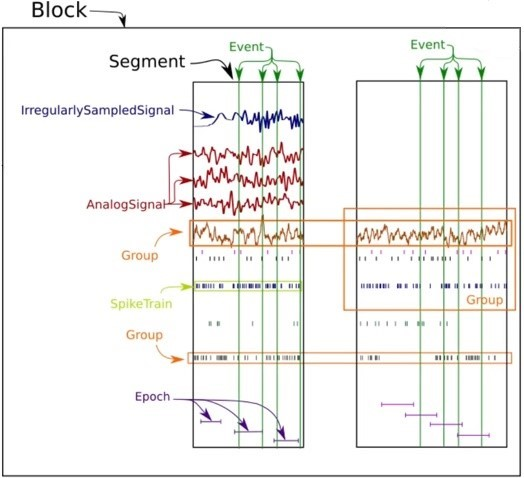
\includegraphics[width = \textwidth]{src/pic/neo_structure}
	\caption{Structure of Neos hierarchical model for electrophysiological data.}
	\label{fig:neostructure}
\end{figure}

\subsection{Custom Structure}
Part of my analysis is still using code from version 1 from openMNGlab where the Neo structure was not yet integrated. The importer from that version delivered the data in a custom data structure.\\
At its core the custom data structure models the data hierarchically, but the objects look a little different from the ones from Neo. At the base level there are data objects "ActionPotential", "MechanicalStimulus", "ElectricalStimulus" containing information corresponding to their respective names. These objects are all part of an overlying object type called $signal_artifact$.\\
On the top level we get an object called "recording" when importing data with this method. one such $recording$ then contains the lists $el_stimuli$, $mech_stimuli$, $actpots$ which are lists containing objects of types $ElectricalStimulus$, $MechanicalStimulus$ and $ActionPotential$ respectively. Additionally there is a $raw_signal$ object which contains the raw signal in the form of arrays.

\section{Development Process}
The basis of my analysis notebook started with the work of Radomir Popovich, who also worked with spike train data for IMI. He had developed a jupyter notebook based on a custom import of spike train data extracted from the Spike2 software. From this he extracted the spike trains and created figures such as event plots(TODO: add event plot figure). These event plots depict the spike trains of a single recording. Each row contains the time point data of spikes for one spike train. The x axis represents the time since the last mechanical stimulus starting at 0. These figures give a good overview with one glance over the spiking sctivity during mechanical stimulation for recordings.

\section{Finished analysis pipeline}
The software development described in the previous chapter resulted in a single jupyter notebook, which represents the current analysis pipeline for this thesis. A schematic version of this pipeline can be seen in figure TODO. The import of the data consists of two separate importing steps. We need to import two files for each data set that contain the information in a slightly different way. 
The first file is the original recording file for spike2. 

\begin{comment}
-Use-cases:\\
	\null\quad-opening data (importing)\\
	\null\quad-latency study (Alina)\\
	\null\quad-chemical data study (Jessica)\\
	\null\quad-mechanically evoked spike trains (Alexander)\\
	\null\quad-experimental researchers (Barbara)\\
-results in a list of requirements\\
-Use-cases lead to software engineering approach\\
-nessecary steps for my analysis\\
-how I implemented it
\end{comment}

\section{Use Cases}
To end this chapter I want to present a couple different use cases of various users of openMNGlab. I will describe the specifics of each use case and then give a few remarks on the current state of openMNGlab and the potential improvements necessary for a smoother experience for all users.

One important feature of openMNGlab that is needed in every use-case is the importing of new data. For new users it is important to be able to load sample data sets and get a feel for the framework by getting to know a few test analysis functions. For students or experimental researchers it is key to be able to load multiple files for a quick overview or even full analysis.\\
Because we are dealing with a couple of different sources when it comes to experimental data, which all need to be handled in a different way, this is where many issues can occur. When going through the use cases we will see where already we encounter some difficulties regarding the data import.



\begin{comment}
-spike2 does some automatic spike filtering
-This results in up to 20 different classes of spikes in one recording
-not all of these, however, are in fact coming from different sources
-experimental researchers have already done their own filtering with their expertise, in order to combine various different of the spike2 classified spikes into larger groups and put them in so called wavemark channels.
-previously one could export these wavemark channels to csv files and inport those into the framework
-with the direct importer from the smr files, however, this is no longer possible
-what we receive after a successful import of an smr recording file are the original spike2 classified spikes in different channels
-if one were to know which of these belong together one could easily combine those together as in spike2 with the wavemark channels
-but the information of the wavemark channels is lost during the import and so one has to manually search for the correct channels first and then combine them into groups by hand
\end{comment}

\subsection{Student 1}
\begin{comment}
Alina \\
Works with spike2 data \\
Electrical data and mechanical data \\
Uses old way of importing currently (csv export from spike2) \\
Needed channels from csv export: \\
DigMark for electrical and mechanical stimulus events \\
WaveMark channel for timestamps of spikes \\
Information used: \\
Electrical stimulus events + timestamps \\
Calculate Latency for spikes (timestamps) \\
Calculate Spike Count  \\
In theory this information is available with the direct import of openMNGlab right now \\
Potential problems with direct openMNGlab importer: \\
Each template for spikes in spike2 results in separate channel in Neo structure after openMNGlab import -> needs some filtering (manual right now) \\
Electrical and mechanical events share a channel (DigMark) and somehow need to be distinguished if the recording also features mechanical stimulation \\
\end{comment}

The first user is a student who does data analysis on mechanically and electrically stimulated Spike2 data. The goal is to perform latency analysis for spikes.  The raw spike2 files feature a lot of information, not all of which is always needed. In this case, all that is required to analyse the latencies of the spikes are the timestamps of the spikes itself and the timestamps of the stimulation events. For the Spike2 software this means that we need to extract the DigMark channel which contains the event information as well as the corresponding wavemark channel which contains the information on the already presorted spikes.\\
The relevant information can be imported using the importing function of openMNGlab. 
The data is then used to calculate the latency for the spikes corresponding to the latest electrical stimulus event as well as calculating the spike count.

Potential problems: The student started the analysis before the framework was working properly and therefore uses their own custom analysis notebook. However, all the information that is required is also available with the regular Spike2 importer in the current openMNGlab version.
In recordings with both electrical and mechanical stimuli, the event markers for those stimuli share the same channel in Spike2. Although they can be distinguished in Spike2 itself, the imported channel in the Neo format does not distinguish between different event types. This needs to be addressed if we want to work with recordings that feature multiple types of stimulation.
Additionally there might be some general import difficulties which I will elaborate on later in this section.
 
\subsection{Student 2}
\begin{comment}
Alexander \\
Works with spike2 data \\
Electrical and mechanically stimulated data \\
Uses a mixture of old and new importing currently \\
Needed channels from csv export: \\
Mechanical force channel \\
Spike channel for timestamps of spikes \\
Need channels from direct spike2 import: \\
Electrical stimulus channel \\
Information used: \\
Electrical stimulus events + timestamps \\
Mechanical stimulus events (duration, amplitude) + timestamps \\
Timestamps for spikes in spike trains \\
Potential problems with the Neo importer: \\
Each template for spikes results in separate spike channels in the Neo structure -> this means that the filtered spikes in the spike2 spike channels (e.g., nw-1…) need to be bundled together again \\
Mechanical force channel import does not work currently \\
Electrical and mechanical events share a channel (DigMark) and somehow need to be distinguished \\
After the import of the mechanical force channel, the mechanical stimuli need to be filtered as such (probably will not happen automatically by the importer) \\
\end{comment}

The second user is also a student who uses mechanically and electrically stimulated Spike2 data. Their goal is to analyse spike trains resulting from mechanical stimulation. For this they do not need all of the information contained in the raw Spike2 file. They need the event information for mechanical and electrical stimuli as well as the mechanical force information for details of the mechanical stimuli. The event information can be found in the DigMark channel of the Spike2 file and gets extracted by the Spike2 importer of openMNGlab. The mechanical force is a continual signal but appears in the form of sin shapes when the nerve is stimulated.
Just as the first user they also need the information regarding the spikes themselves, which are also imported by the framework.\\
From the gathered data the user then calculates various quantifiers for the mechanically induced spike trains such as spike count or more elaborate features. The user started this project while still using the old framework version where the channels from the Spike2 software were manually extracted to a csv file. With the updates to the framework in the meantime not all of the required information gets extracted as easily as before. This is why they use a hybrid version of the two versions of the framework where they mix and match the functions as they need them.
%it is probably clear that this user is me. Should I just say so?

Potential problems: There are similar potential problems when it comes to the event channels and regular spike channels as in the case of the first user. Additionally there are problems when it comes to the import of the mechanical force. The user started the analysis with an old version of the framework which used other importers (csv files). With this technique they could extract the mechanical force throughout the recordings. The new Neo importer still has some bugs when it comes to importing the mechanical force from the Spike2 file, which requires fixing for future users who need this information.

\subsection{Student 3}
\begin{comment}
Jessica \\
Works with spike2 data \\
Chemical data \\
Uses Neo importer \\
Needed channels from import: \\
Spike channels for spike timestamps \\
Information used: \\
Intervals which are relevant for the application of chemicals \\
Spikes + timestamps inside those intervals \\
Which chemicals are applied when \\
Potential problems with openMNGlab importer: \\
The chemical protocols are not automatically importable and readable; There is a channel in spike2 for comments where this information is given in theory, however, the notation of what is given and how much varies from comment to comment, and one needs a good understanding of the chemicals and potentially experimental procedure \\
Comments channel is not being imported currently, even if the chemical notes where uniform; This means one must manually reed the comment channel in the spike2 software itself and manually choose some intervals which might be promising for observing chemically induced changes in spiking activity \\
\end{comment}

The third student user of the framework works on a project to analyse Spike2 data in which certain chemicals where applied to the test subject. In contrast to the other two users, this user started with the project when the current version of openMNGlab with the integration of the Neo module already in place. This means they only made use of the new importing functions and are not stuck with certain parts from the old framework. In addition to the spiking activity, as in the previous use-cases, they also need information regarding the chemicals that are applied. They need the timings and doses of the specific chemicals. From this they need to specify a time frame where they want to monitor the spiking activity that results from the application of the chemicals.\\

Potential problems: The analysis of chemically stimulated data does bring with it its own new set of problems. There is no dedicated channel for chemical information in the Spike2 software. For this reason the chemical protocols are given in the general comment channel in Spike2. That means that the experimenter manually creates a comment every time a new chemical is applied. The issue with this is that openMNGlab does not import the comment channel. In practice the comments do not have a strict naming scheme, which would also lead to difficulties with the automatic detection of specifics regarding the chemicals. This is a problem however that does not stem from the framework, but is something that has to be addressed on the side of the experimental researchers.\\
These described problems lead to the current workflow of manually selecting a suitable time frame for interesting spiking activity some time after the chemical application; some times up to a minute (check the times again) after the chemicals where applied.

\subsection{Experimental researcher}
Another big group of potential users for openMNGlab are experimental researchers who produce and work with electrophysiological and microneurographical data often. They will be a big part of the user base of the framework because of the nature of their work. For them it is important that the new data sets can be easily and quickly loaded and overview statistics can be displayed.


 
\begin{comment}
Which information should available after importing data? \\
Spikes + timestamps \\
Electrical stimulation + timestamps \\
Mechanical stimulation + timestamps, duration, amplitude \\
Information about application of other stimuli (chemicals, heat…) \\
For human data: temperature?  

Spike2 \\
Spike channels + some way to group them easily (e.g., in groups from spike2 templates) \\
Electrical event channel + some way to distinguish between electrical and mechanical events \\
Mechanical force channel (maybe optional) \\
Comments channel (maybe optional) \\
Temperature (optional) (probably needed for human data) \\
\end{comment}

\begin{comment}
My steps in analysis: 

First, I used a jupyter notebook from Radomir. For this the data needed to be extracted from Spike2 directly in the Software. This export step leads to a single csv file for one recording with 5 channels: Time, Signal, Force, DigMark(stimulation events), Spikes 

Using the csv files I could extract the spike trains for each mechanical stimulation. The detection of the spike train worked as follows: The start of the spike train gets determined by the stimulation event. The length of the spike train is a previously set amount of time (in most cases 500ms). During this timeframe all spikes in the spike channel get put into a list that keeps track of the spike trains. This pretty basic detection of spike trains works well in this specific use case but has its limits when it comes to other kinds of data with other experimental protocols or just simply recordings without any protocols. Then because we do not have the exact starting points of the trains or bursting patterns this method of detection falls flat. 

This first jupyter notebook already made use of what later became openMNGlab. The import of the data was handled by the software framework. However, openMNGlab got some updates soon after which made some significant changes to how the importers work. In the new and improved framework, the importer worked on the original Spike2 files instead of the extracted csv files. This allows for more detailed representation of the data since much of the information was lost in the extraction before this update. However, with this new way of importing the data the mechanical stimulation was not able to be extracted. I still needed the information of the mechanical stimulation which was only contained in the extracted csv file. For this reason, in my analysis from here on, I used a hybrid of the old and new versions of openMNGlab until I was able to fix the new importer to also include the mechanical stimulation channel. 
\end{comment}

\cleardoublepage
